\documentclass[11pt]{article}

\input{preamble/preamble.tex}
\input{preamble/preamble_math.tex}
\input{preamble/preamble_acronyms.tex}

\newcommand{\celegans}{\textit{C. elegans}}

% \title{\large Discrete and continuous latent states of neural activity in \textit{Caenorhabditis elegans}}
\title{Hierarchical recurrent models reveal latent states of neural activity in \textit{C. elegans}}
\author{Scott Linderman$^{\text{1}}$,
  Annika Nichols$^{\text{2}}$,
  David Blei$^{\text{1}}$,
  Manuel Zimmer$^{\text{2}}$,
  and
  Liam Paninski$^{\text{1}}$
  \\
  $^{\text{1}}$Columbia University,
  $^{\text{2}}$Research Institute of Molecular Pathology (IMP), Vienna Biocenter
}

\begin{document}

\doublespacing

\maketitle

\begin{abstract}
  Recent advances in neural recording technologies have enabled
  simultaneous measurements of the majority of head ganglia neurons in
  both immobilized and freely-behaving
  \celegans~\citep{schrodel2013brain, prevedel2014simultaneous,
    nguyen2016whole}.  The dynamics of neural activity shed light on
  how \celegans~processes sensory information and generates motor
  activity.  To understand these dynamics, we develop recurrent state
  space models that decompose complex time-series into segments with
  simple, linear dynamics. We incorporate these models into a robust,
  hierarchical framework for combining information across whole-brain
  recordings of many worms.  Using this framework, we reveal latent
  states of population neural activity, along with the discrete
  behavioral modes that drive dynamics in this latent state space.  We
  find stochastic transition patterns between these discrete
  behavioral modes, and we see that transition probabilities are
  determined by a combination of current brain state and environmental
  cues.  In addition to quantifying neural dynamics, this
  probabilistic framework aids in neural identification---currently a
  laborious, manual task---and reveals clusters of neurons that are
  similarly tuned in latent state space.  Finally, we find a
  significant overlap between our inferred modes and the
  manually-labeled modes of~\citet{kato2015global}
  and~\citet{nichols2017global}, which were shown to correspond to
  different behaviors, like forward crawling, reversals, and
  turns. Our methods automatically discover and quantify these
  behaviorally-meaningful states directly from neural activity,
  yielding powerful new tools for neuro-behavioral analysis.
\end{abstract}

\clearpage

\section*{Introduction}

\clearpage

\section*{Results}

\subsection*{A probabilistic framework that combines information across
  trials to learn canonical dynamics}

\begin{figure}[ht]
\centering%
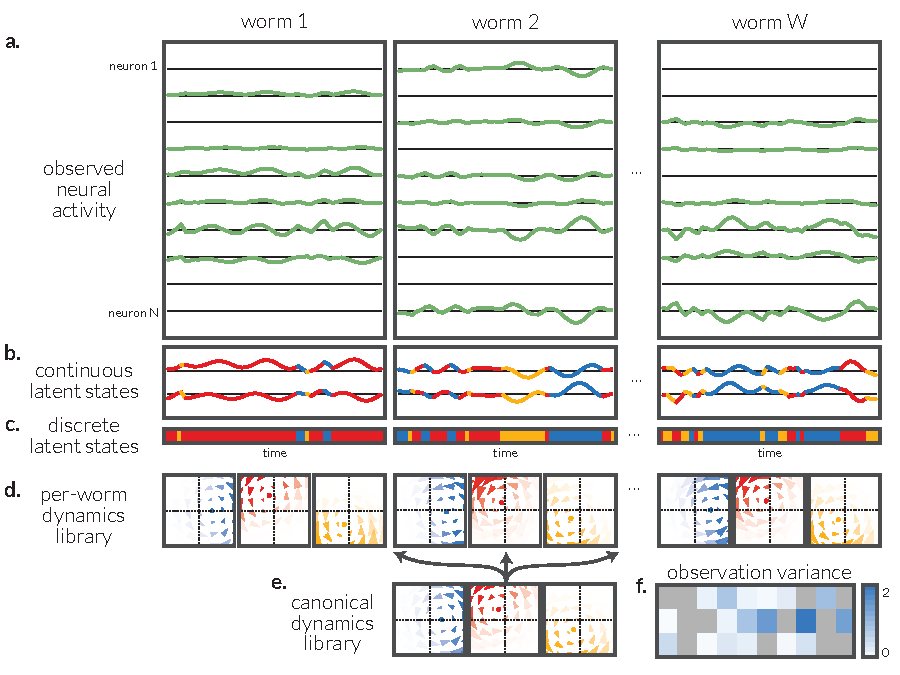
\includegraphics[width=6in]{figures/figure1} 
\caption{A schematic of the hierarchical model for combining
  information across multiple worms in order to learn a shared
  dynamical system for \celegans.  \textbf{a.}~All worms share a
  canonical dynamics library. Here, we have three dynamics functions
  (blue, red, gold), each of which is a simple linear mapping from
  $x_t \in \reals^2$ to $x_{t+1} \in \reals^2$.  The recurrent model
  assigns probabilities to the different dynamics functions based on
  the current location in $x$-space.  \textbf{b.}~The worms also share
  an emission matrix, $C$, which can be viewed as an embedding of
  neurons in latent space.  \textbf{c.}~Each worm has its own dynamics
  library, which allows for slight deviations from the canonical
  dynamics.  \textbf{d.}~The model segments neural activity into a
  sequence of discrete states~$z_{t} \in \{1, 2, 3\}$, which index
  into the dynamics library.  \textbf{e.}~The discrete states specify
  the dynamics that are used to propagate the continuous latent
  states~$x_t$ forward in time. Here, the two dimensional latent
  states are colored according to the instantaneous discrete
  state. \textbf{f.}~The observed neural activity is a linear
  projection of the underlying continuous latent states.  On any given
  trial, we observe only a fraction of all the neurons.  The
  hierarchical model combines these partial recordings to infer the
  underlying states, the dynamics libraries, and the shared neural
  embedding. }
\label{fig:model}
\end{figure}

We seek a parsimonious characterization of the dynamics of neural
activity in the head ganglia of \celegans. Recent advances in optical
imaging offer simultaneous recordings of most of the head ganglia
neurons, but we must surmount three main challenges in order to learn
a dynamics model from these data.  First, we need to design a model
flexible enough to capture nonlinear dynamics yet interpretable enough
to reveal simplifying structure when it exists.  Moreover, any model
will necessarily be an approximation to the true neural dynamics, and
as such we need to be robust to data that does not quite match model
predictions.  Finally, our model must combine partial recordings from
separate organisms to learn shared neural dynamics yet still allow for
individual variability. We construct a recurrent, robust, and
hierarchical state space model that addresses these challenges,
decomposing complex dynamics into a collection of simpler pieces that
can be learned from noisy, partial recordings with trial-to-trial
variability.

We study the data presented in~\citet{kato2015global} and
\citet{nichols2017global}, which consist of a collection of optical
recordings of calcium fluorescence in immobilized \celegans. The
recordings are 18 minutes long with a frame rate of about 3Hz.  On
average, about 100 single units are extracted from each
recording. \celegans~is genetically stereotyped and each of its 302
neurons has a unique label (e.g. \textsf{AVAL}). On average, 30 single
units could be unambiguously labeled in each
recording. Fig.~\ref{fig:model}a illustrates this type of data. The
three panels represent recordings from three separate worms, and the
rows correspond to different neuron labels.  Neural activity is
measured for only a subset of neurons in each worm.

% To model this data, we build on switching linear dynamical systems
% (SLDS) \citep{chang1978state, ackerson1970state, hamilton1990analysis,
%   ghahramani1996switching, murphy1998switching}, a type of state space
% model that views data as a projection of a low-dimensional latent
% state that switches between linear dynamical regimes.  Formally,
% let~$y_t \in \reals^N$ denote the vector of neural activity observed
% at time~$t$.  The expected activity is given by,~$\E[y_t] = g(x_t)$,
% where~$x_t \in \reals^D$ is a continuous latent state
% and~$g: \reals^D \to \reals^N$ is a linear map. We assume~$D \ll N$,
% reflecting the low-dimensional nature of neural activity. SLDS
% simplify the dynamics of the continuous latent states by introducing a
% discrete latent state~$z_t \in \{1, \ldots, K\}$ that indicates the
% current dynamical regime.  Each discrete regime~$k$ is associated with
% a linear map~$f_k: \reals^D \to \reals^D$. The discrete state~$z_t$
% specifies which map to use in order to propagate~$x_t$ to the next
% time step.  Specifically,~$\E[x_{t+1}] = f_{z_t}(x_t)$. By switching
% between different linear dynamical regimes, the SLDS captures highly
% nonlinear dynamics.  We seek to infer the continuous and discrete
% latent states and simultaneously learn the linear maps, the
% distribution of the noise in the observations and the continuous
% states, and the dynamics that govern how the discrete latent states
% evolve.
To model this data, we build on switching linear dynamical systems
(SLDS) \citep{chang1978state, ackerson1970state, hamilton1990analysis,
  ghahramani1996switching, murphy1998switching}, a type of state space
model that views data as a projection of a low-dimensional latent
state that switches between linear dynamical regimes.  The expected
activity is a linear function of an underlying, continuous latent
state, illustrated as two-dimensional time series for each worm in
Fig.~\ref{fig:model}b.  We typically assume this latent state is lower
dimensional than the number of observed neurons. SLDS simplify the
dynamics of the continuous latent states by introducing discrete
latent states that indicate the current dynamical regime
(Fig.~\ref{fig:model}c).  Each discrete regime is associated with a
linear map (Fig.~\ref{fig:model}d), and the discrete state specifies
which map to use in order to propagate the continuous latent state to
the next time step.  By switching between different linear dynamical
regimes, the SLDS captures highly nonlinear dynamics.  We seek to
infer the continuous and discrete latent states and simultaneously
learn the linear maps, the distribution of the noise in the
observations and the continuous states, and the dynamics that govern
how the discrete latent states evolve.

% Recurrent model
Standard SLDS treat the discrete latent states as a simple Markov
process: the next state depends only on the current state. However,
this neglects the more nuanced ways in which discrete and continuous
states may co-evolve. For example, the next discrete state may depend
on both the current discrete state and the current location in
continuous latent space; intuitively, different dynamical regimes may
be employed in different regions of continuous latent space. These
types of dependencies are captured by what are variously called
hybrid~\citep{paoletti2007identification},
augmented~\citep{barber2006expectation}, or \emph{recurrent} state
space models~\citep{linderman2017recurrent}. The maps in
Fig.~\ref{fig:model}d illustrate how these dependencies may modulate
the probability of different dynamics depending on the current
location in continuous latent space. We employ these recurrent models
to learn dynamical regimes that are selectively employed as a
function of current continuous brain state.

% Robust model
While recurrent SLDS can approximate highly nonlinear systems, they
are still misspecified. \emph{Robust} methods~\citep{huber1981robust}
ameliorate this concern by lessening the penalty on observations that
do not quite match the dynamics of the current regime.  We achieve
this robustness by replacing the standard Gaussian noise model with a
multivariate-t distribution~\citep{lange1989robust}.  The heavy tails
of this distribution permit outliers and account for some of the model
misspecification.

% Hierarchical model
The third component of our framework is a \emph{hierarchical} model
for learning canonical dynamics from partial recordings collected from
many worms.  Since each recording contains a different subset of
labeled neurons, our first step is to align the data, treating the
activity of neurons that were not found in a given recording as
missing data that must be inferred.  We handle this by integrating
over possible activity of the missing neurons, analytically
marginalizing out this missing data.  The second challenge is
combining information from many recordings while also allowing for
worm-to-worm differences.  For example, the neural activitiy may have
larger variance in some recordings than in others due to different
levels of expression of the fluorescent protein.  We allow for this by
having a separate variance for each worm and neuron, as shown in
Fig.~\ref{fig:model}f.  More importantly, the dynamics of neural
activity may be slightly different from worm to worm.  We account for
this by introducing a canonical library of dynamical regimes
(Fig.~\ref{fig:model}e) that are shared by all worms as well as a
unique library for each individual worm (Fig.~\ref{fig:model}d);
however, we constrain the per-worm dynamics to be close to the
canonical dynamics.


\subsection*{Emission models reveal clusters of neurons and aid in identification}

\begin{figure}[t]
\centering%
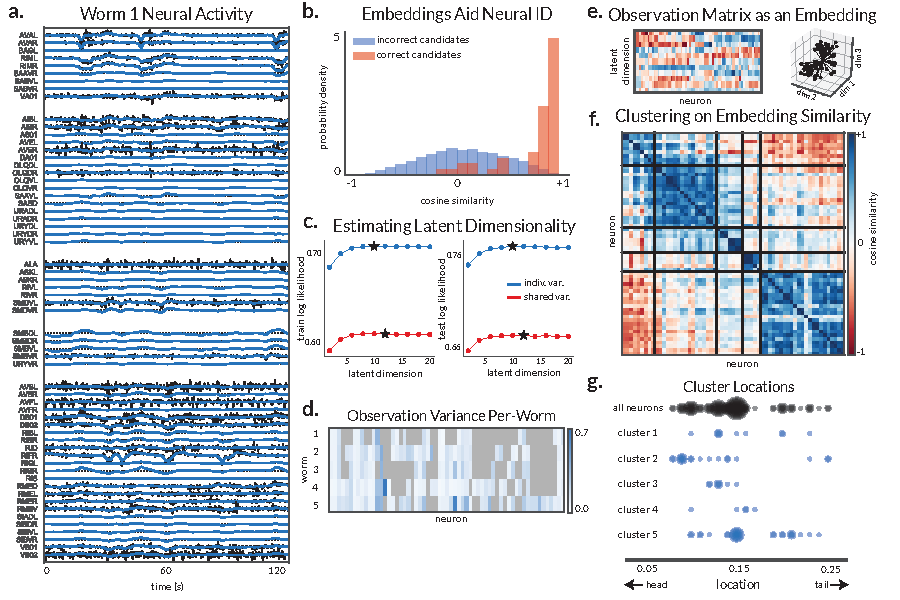
\includegraphics[width=6in]{figures/figure2} 
\caption{}
\label{fig:emissions}
\end{figure}


\subsection*{SLDS automatically parse data into discrete states with simple dynamics}

\begin{figure}[t]
\centering%
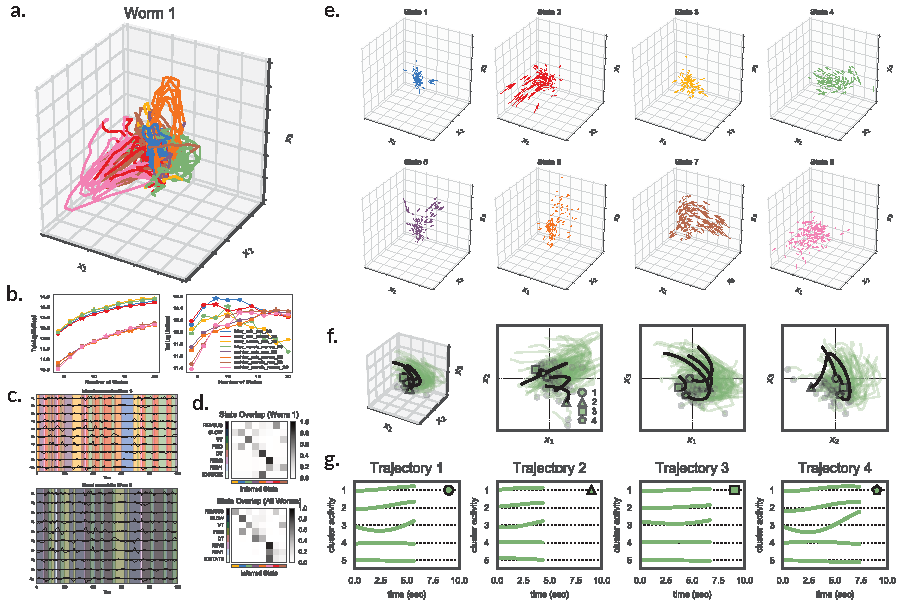
\includegraphics[width=6in]{figures/figure3} 
\caption{}
\label{fig:syllables}
\end{figure}

\subsection*{Recurrent models learn spatially localized states and transition boundaries}

\begin{figure}[t]
\centering%
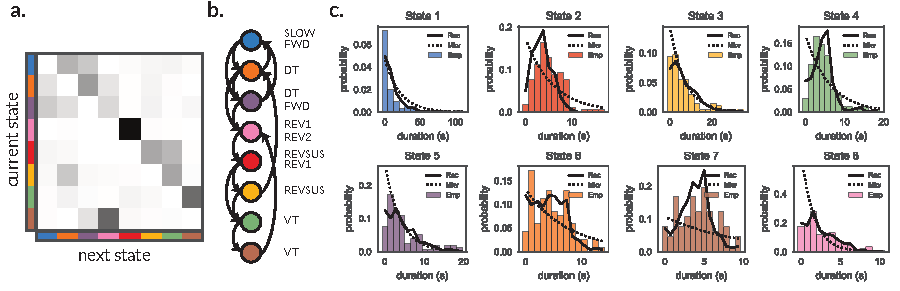
\includegraphics[width=6in]{figures/figure4} 
\caption{}
\label{fig:recurrent}
\end{figure}

\subsection*{Oxygen level modulates transition probabilities but not dynamics or emissions}

\begin{figure}[t]
\centering%
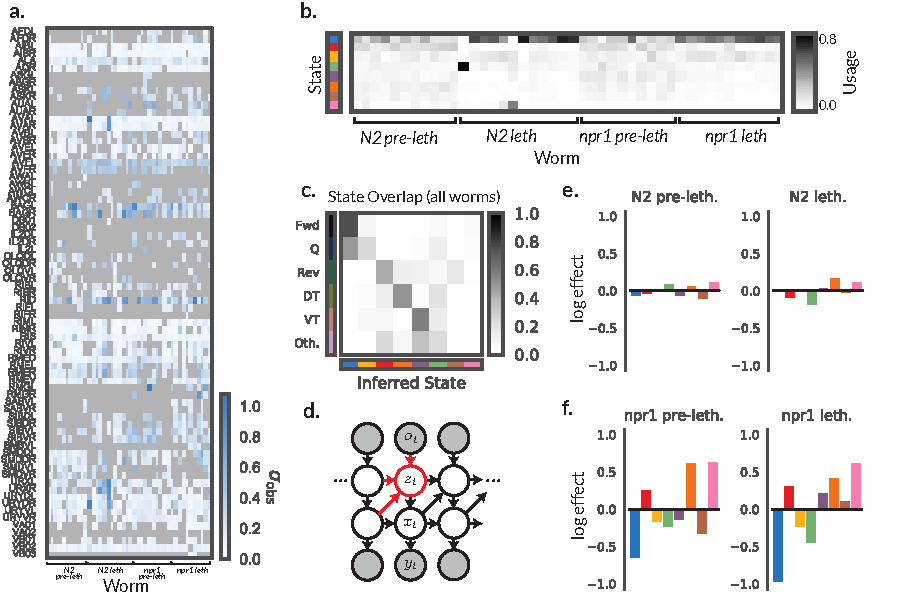
\includegraphics[width=6in]{figures/figure5} 
\caption{}
\label{fig:o2}
\end{figure}


\clearpage

\section*{Discussion}

\clearpage

\bibliography{refs}
\bibliographystyle{abbrvnat}

\clearpage

\appendix

\section{Data}
\label{sec:data}

The data comes in the form of a collection of matrices~$\{\widetilde{Y}^{(w)}\}_{w=1}^W$
for each of~$W$ worms.  The matrix~${\widetilde{Y}^{(w)} \in \reals^{T_w \times N_w}}$
represents the calcium activity of the~$w$-th worm, which consists of~$T_w$
time frames and~$N_w$ neurons.\footnote{Technically, this calcium activity is
a matrix of first-order temporal differences of a
bleaching-corrected~$\Delta F /F$ signal. Unlike~\citet{kato2015global}, we
do not smooth these derivatives. We work with the raw first-order
temporal differences.}  \celegans~is special in that each neuron has a unique
name.  Assigning names to neurons in calcium imaging data is a challenging
task, but typically, out of the~${\sim 100}$ neurons observed in any worm,
we can label about~$20-30$ with high certainty.  As such, we choose to
represent each matrix~$\widetilde{Y}^{(w)}$ in \emph{canonical form} as a
tuple~$(Y^{(w)}, M^{(w)})$, where~${Y^{(w)} \in \reals^{T_w \times N}}$ is
a matrix where each column corresponds to one of the~$N$ neurons that is
identified in at least one of the~$W$ worms, and~${M^{(w)} \in \{0,1\}^{T_w \times N}}$
is a corresponding \emph{mask} matrix that indicates which neurons were
observed in worm~$w$.  If~$M_{:,n}^{(w)} = 1$, neuron~$n$ was labeled in
worm~$w$ and~$Y_{:,n}^{(w)}$ was its observed activity.  If~$M_{:,n}^{(w)}=0$,
this neuron was not observed in worm~$w$, and the corresponding activity
is missing.\footnote{The mask is defined in such a way that neurons can
  be missing for only subsets of time frames, but in our data neurons are
  either labeled or missing.}
% todo: note that we could also (and have also) model the activity of
% unlabeled neurons.  For the final analyses, I'm not doing this though.

\section{Hierarchical Generative Model}

We model the neural activity with a switching linear
dynamical system (SLDS) with three new extensions: (i)~a \emph{hierarchical} model
to share parameters across worms while also allowing for worm-to-worm
variability; (ii)~a \emph{robust} model for dynamics noise to help address
model misspecification; and (iii)~a \emph{recurrent} model to capture
how continuous latent states influence discrete state transition probabilities.
We will introduce the SLDS first and then present each of these extensions
in turn.


\subsection{Switching linear dynamical systems}
\label{sec:slds}
Switching linear dynamical system models (SLDS) break down complex, nonlinear
time series data into sequences of simpler, reused dynamical modes.
By fitting an SLDS to data, we not only learn a flexible nonlinear generative
model, but also learn to parse data sequences into coherent discrete units.

The generative model is as follows. At each time ${t=1,2,\ldots,T}$,
for each worm~$w$,
there is a discrete latent state ${z_t^{(w)} \in \{1,2, \ldots,K\}}$ that
follows Markovian dynamics,
\begin{equation}
  z_{t+1}^{(w)} \given z_t^{(w)}, \{\pi_k\}_{k=1}^K  \sim \pi_{z_t^{(w)}}
  \label{eq:markov_z}
\end{equation}
where ${\{\pi_k\}_{k=1}^K}$ is the Markov transition matrix and
${\pi_k \in [0,1]^K}$ is its $k$th row. 
In addition, a continuous latent state ${x_t^{(w)} \in \reals^D}$ follows
conditionally linear (or affine) dynamics, where the discrete state $z_t^{(w)}$
determines the linear dynamical system used at time $t$:
\begin{align}
  x_{t+1}^{(w)} &= A_{z_{t+1}^{(w)}} x_{t}^{(w)} + b_{z_{t+1}^{(w)}} +  u_t^{(w)},
  &
  u_t^{(w)} &\iid\sim \cN(0,Q_{z_{t+1}^{(w)}}),
  \label{eq:slds_start}
\end{align}
for matrices ${A_k, Q_k \in \reals^{D \times D}}$ and vectors~${b_k\in
\reals^D}$ for~${k=1,2,\ldots,K}$.
Finally, at each time $t$ a linear Gaussian observation $y_t^{(w)} \in \reals^N$
(some entries of~$y_t^{(w)}$ are masked off; recall Section~\ref{sec:data}) is
generated from the corresponding latent continuous state,
\begin{align}
  y_t^{(w)} &= C x_t^{(w)} + d + v_t^{(w)}, & v_t^{(w)} &\iid\sim \cN(0,S),
    \label{eq:slds_end}
\end{align}
for $C \in \reals^{N \times D}$, $S \in \reals^{N \times N}$,
and~$d \in \reals^N$. We denote the rows of~$C$ by vectors~$c_n$.
For simplicity, we assume~$C$,~$d$, and~$S$ to
be shared among all discrete states in our model.  Moreover, we assume
the observation noise is diagonal,
\begin{align*}
  S &= \diag\left(\left[s_{1}, \ldots, s_{N} \right] \right). 
\end{align*}
The system parameters comprise the discrete Markov transition matrix, the
library of linear dynamical system matrices, and the neuron-specific
emission parameters, which we write as
\begin{equation*}
  \theta = \{(\pi_k, A_k, Q_k, b_k)\}_{k=1}^K \cup \{c_n, d_n, s_n\}_{n=1}^N.
\end{equation*}

To learn an SLDS using Bayesian inference, we place conjugate Dirichlet priors
on each row of the transition matrix and conjugate matrix normal
inverse Wishart (MNIW) priors on the linear dynamical system parameters,
Gaussian priors on the rows of the emission matrix,
and inverse gamma priors on the emission noise.
We write this as,
\begin{align*}
  \pi_k &\given \alpha \iid\sim \distDirichlet(\alpha),
  &
  [A_k, b_k], Q_k &\given \lambda \iid\sim \distMNIW(\lambda),
  \\
  [c_n, d_n] &\given \eta \iid\sim \distNormal(\eta),
  &
  s_{n} &\given \eta \iid\sim \mathrm{IG}(\eta).
\end{align*}
where~$[\cdot, \cdot]$ denotes column concatenation, and $\alpha$, $\lambda$,
and~$\eta$ denote appropriate hyperparameters of the transitions, dynamics, and
emissions, respectively.


\end{document}
